% main_revised.tex — revised manuscript source (2026-10-20)
% (Claude Code) at the researcher's request; logged in docs/integrity/AI_ASSISTANCE_LOG.md. The researcher's main.tex is
% unchanged. What changed: multiverse title restored; "supplied/source-reported" hedging removed (the pre-registration
% commits, run manifests and per-query results are in the repository); every number is a macro from numbers.tex and
% every results table is generated (tables/*.tex); citations use the verified bibliography (refs.bib); AI-use
% statement restored. The reconstruction's precise wording on estimands, budgets and limits is kept.
%
% Build: python -I manuscript/make_numbers.py; python -I manuscript/make_tables.py;
%        .venv/bin/python -I manuscript/make_bib.py; latexmk -pdf main_revised.tex
% \citeL{key}: cited work not yet read in full (below L3) -> red dagger. None may remain at submission.
% \todo{...}: something only the researcher can supply.
\documentclass[11pt]{article}
\usepackage[margin=1in]{geometry}
\usepackage[T1]{fontenc}
\usepackage[utf8]{inputenc}
\usepackage{lmodern,microtype}
\usepackage{booktabs,graphicx,amsmath,amssymb,array,tabularx}
\usepackage{xcolor,enumitem,caption,placeins}
\usepackage[numbers,sort&compress]{natbib}
\usepackage[hidelinks]{hyperref}
\usepackage{xurl}
% Generated by manuscript/make_numbers.py from logged results. Do not edit by hand.
\newcommand{\AuditBudget}{1}
\newcommand{\AuditExposed}{9}
\newcommand{\AuditExposedHi}{68.3}
\newcommand{\AuditExposedLo}{27.3}
\newcommand{\AuditExposedPct}{47.4}
\newcommand{\AuditFixedK}{12}
\newcommand{\AuditN}{19}
\newcommand{\AuditUncertainty}{3}
\newcommand{\EoneNq}{9,253}
\newcommand{\EoneNqCovidqa}{1,771}
\newcommand{\EoneNqCuad}{996}
\newcommand{\EoneNqQasper}{1,742}
\newcommand{\EoneNqSquadtwo}{4,744}
\newcommand{\EtwoEmFiveTwelveBudget}{0.125}
\newcommand{\EtwoEmFiveTwelveCount}{0.090}
\newcommand{\EtwoEmOneTwoEightBudget}{0.085}
\newcommand{\EtwoEmOneTwoEightCount}{0.105}
\newcommand{\EtwoJobsCuad}{400}
\newcommand{\EtwoJobsQasper}{400}
\newcommand{\EtwoPoneCov}{+0.089}
\newcommand{\EtwoPoneCovHi}{+0.132}
\newcommand{\EtwoPoneCovLo}{+0.050}
\newcommand{\EtwoPoneCovMde}{0.059}
\newcommand{\EtwoPoneEm}{\ensuremath{-}0.055}
\newcommand{\EtwoPoneEmHi}{\ensuremath{-}0.010}
\newcommand{\EtwoPoneEmLo}{\ensuremath{-}0.100}
\newcommand{\EtwoPoneEmMde}{0.066}
\newcommand{\EtwoPoneFone}{\ensuremath{-}0.017}
\newcommand{\EtwoPoneFoneHi}{+0.033}
\newcommand{\EtwoPoneFoneLo}{\ensuremath{-}0.065}
\newcommand{\EtwoPoneFoneMde}{0.068}
\newcommand{\EtwoPoneFoneMdeStrat}{0.068}
\newcommand{\EtwoSquadFiveTwelveBudgetCov}{0.88}
\newcommand{\EtwoSquadFiveTwelveBudgetFone}{0.58}
\newcommand{\EtwoSquadOneTwoEightBudgetCov}{0.86}
\newcommand{\EtwoSquadOneTwoEightBudgetFone}{0.44}
\newcommand{\EtwoSthreeCov}{+0.035}
\newcommand{\EtwoSthreeCovHi}{+0.060}
\newcommand{\EtwoSthreeCovLo}{+0.015}
\newcommand{\EtwoSthreeCovMde}{0.036}
\newcommand{\EtwoSthreeEm}{\ensuremath{-}0.015}
\newcommand{\EtwoSthreeEmHi}{+0.020}
\newcommand{\EtwoSthreeEmLo}{\ensuremath{-}0.050}
\newcommand{\EtwoSthreeEmMde}{0.051}
\newcommand{\EtwoSthreeFone}{+0.004}
\newcommand{\EtwoSthreeFoneHi}{+0.036}
\newcommand{\EtwoSthreeFoneLo}{\ensuremath{-}0.024}
\newcommand{\EtwoSthreeFoneMde}{0.044}
\newcommand{\EtwoTruncCuad}{65}
\newcommand{\EtwoTruncQasper}{2}
\newcommand{\HFiveBBudget}{91.7}
\newcommand{\HFiveBCount}{33.3}
\newcommand{\HFiveBEst}{58.3}
\newcommand{\HFiveBHi}{64.6}
\newcommand{\HFiveBLo}{45.1}
\newcommand{\HFiveBVerdict}{supported}
\newcommand{\HFiveBudgetFiveTwelve}{5.6}
\newcommand{\HFiveCountFiveTwelve}{25.0}
\newcommand{\HFiveEst}{19.4}
\newcommand{\HFiveHi}{41.7}
\newcommand{\HFiveLo}{16.7}
\newcommand{\HFiveSeedMax}{24.3}
\newcommand{\HFiveSeedMin}{21.5}
\newcommand{\HFiveSeedN}{9}
\newcommand{\HFiveVerdict}{inconclusive}
\newcommand{\HFourBBudget}{71.3}
\newcommand{\HFourBCount}{6.9}
\newcommand{\HFourBEst}{64.4}
\newcommand{\HFourBHi}{68.3}
\newcommand{\HFourBLo}{56.5}
\newcommand{\HFourBVerdict}{supported}
\newcommand{\HFourBmOnlyBudget}{61.1}
\newcommand{\HFourBmOnlyCount}{0.0}
\newcommand{\HFourBmOnlyEst}{61.1}
\newcommand{\HFourBmOnlyHi}{72.5}
\newcommand{\HFourBmOnlyLo}{57.2}
\newcommand{\HFourBudget}{64.8}
\newcommand{\HFourCount}{9.4}
\newcommand{\HFourDenseOnlyBudget}{68.5}
\newcommand{\HFourDenseOnlyCount}{18.8}
\newcommand{\HFourDenseOnlyEst}{49.8}
\newcommand{\HFourDenseOnlyHi}{58.1}
\newcommand{\HFourDenseOnlyLo}{39.1}
\newcommand{\HFourEst}{55.4}
\newcommand{\HFourHi}{63.1}
\newcommand{\HFourLo}{50.8}
\newcommand{\HFourVerdict}{supported}
\newcommand{\HOneBEst}{26.7}
\newcommand{\HOneBHi}{33.9}
\newcommand{\HOneBLo}{15.4}
\newcommand{\HOneBVerdict}{supported}
\newcommand{\HOneEst}{71.1}
\newcommand{\HOneHi}{81.9}
\newcommand{\HOneLo}{64.8}
\newcommand{\HOneVerdict}{supported}
\newcommand{\HThreeMedianN}{1,256}
\newcommand{\HThreeShare}{85.4}
\newcommand{\HThreeVerdict}{supported}
\newcommand{\HTwoDatasetEta}{0.61}
\newcommand{\HTwoFraction}{100.0}
\newcommand{\HTwoRetrieverEta}{0.04}
\newcommand{\HTwoVerdict}{supported}
\newcommand{\PoneBudgetFiveTwelve}{7.6}
\newcommand{\PoneBudgetOneTwoEight}{81.2}
\newcommand{\PoneCountFiveTwelve}{78.8}
\newcommand{\PoneCountOneTwoEight}{0.0}
\newcommand{\PoneDenseUniversesBudget}{36}
\newcommand{\PoneDenseUniversesCount}{48}
\newcommand{\PoneUniversesBudget}{576}
\newcommand{\PoneUniversesCount}{768}
\newcommand{\PosthocCharFlips}{965}
\newcommand{\PosthocEquivElements}{85,275,648}
\newcommand{\PosthocEquivElementsB}{1,665,540}
\newcommand{\PosthocUniverses}{24,960}
\newcommand{\SemBpMax}{320}
\newcommand{\SemBpMin}{278}
\newcommand{\SemClMax}{458}
\newcommand{\SemClMin}{452}
\newcommand{\SemClNoncontigMin}{92.0}
\newcommand{\SensAllBudgetsEst}{74.2}
\newcommand{\SensAllBudgetsHi}{84.8}
\newcommand{\SensAllBudgetsLo}{68.3}
\newcommand{\SensBHEst}{68.0}
\newcommand{\SensBHPooledEst}{70.4}
\newcommand{\SensClusterEst}{69.7}
\newcommand{\SensClusterHi}{82.0}
\newcommand{\SensClusterLo}{63.8}
\newcommand{\SensDefRetEst}{70.8}
\newcommand{\SensDefRetHi}{85.4}
\newcommand{\SensDefRetLo}{64.6}
\newcommand{\SensNoSquadEst}{61.5}
\newcommand{\SensNoSquadHi}{74.8}
\newcommand{\SensNoSquadLo}{53.2}
\newcommand{\SfiveOneTwoEightBudgetFix}{75.0}
\newcommand{\SfiveOneTwoEightBudgetSem}{8.3}
\newcommand{\SfiveOneTwoEightCountFix}{16.7}
\newcommand{\SfiveOneTwoEightCountSem}{60.4}
\newcommand{\SfiveUniversesBudget}{72}
\newcommand{\SfiveUniversesCount}{96}
\newcommand{\SoneOneTwoEightBudgetA}{60.5}
\newcommand{\SoneOneTwoEightBudgetB}{6.2}
\newcommand{\SoneOneTwoEightCountA}{0.0}
\newcommand{\SoneOneTwoEightCountB}{74.1}
\newcommand{\SoneSixFourBudgetA}{20.0}
\newcommand{\SoneSixFourBudgetB}{42.1}
\newcommand{\SoneSixFourCountB}{84.1}
\newcommand{\StwoOneTwoEightBudgetA}{55.1}
\newcommand{\StwoOneTwoEightBudgetB}{1.9}
\newcommand{\StwoOneTwoEightCountA}{51.6}
\newcommand{\StwoOneTwoEightCountB}{1.8}
\newcommand{\StwoTwoFiveSixBudgetA}{39.8}
\newcommand{\StwoTwoFiveSixBudgetB}{3.3}
\newcommand{\StwoTwoFiveSixCountA}{36.1}
\newcommand{\StwoTwoFiveSixCountB}{3.5}

\newcommand{\pp}{\ensuremath{\,\mathrm{pp}}}
\newcommand{\chunk}[1]{\texttt{#1}}
\newcommand{\ind}{\mathbb{1}}
\newcommand{\citeL}[1]{\cite{#1}\textsuperscript{\textcolor{red}{\dag}}}
\newcommand{\todo}[1]{\textcolor{red}{[TODO: #1]}}
\newcommand{\AuthorName}{}
\newcommand{\AuthorAffiliation}{}
\newcommand{\AuthorEmail}{}
\captionsetup{font=small,labelfont=bf,skip=6pt}
\setlength{\emergencystretch}{2em}
\setlist{nosep}
\renewcommand{\topfraction}{0.92}
\renewcommand{\bottomfraction}{0.85}
\renewcommand{\textfraction}{0.08}
\renewcommand{\floatpagefraction}{0.75}
\setcounter{topnumber}{3}
\setcounter{totalnumber}{5}
\hypersetup{pdftitle={Chunking Verdicts in Retrieval-Augmented Generation Are Artefacts of the Evaluation Protocol: A Pre-registered Multiverse Analysis}}

\title{Chunking Verdicts in Retrieval-Augmented Generation Are Artefacts\texorpdfstring{\\}{ }of the Evaluation
Protocol: A Pre-registered Multiverse Analysis}
% Complete these fields after confirming authorship and submission anonymity.
\author{\AuthorName}
\date{}
\makeatletter
\renewcommand{\@maketitle}{%
  \begin{center}
    {\LARGE \@title\par}
    \ifx\AuthorName\@empty\else
      \vskip 0.8em {\large \AuthorName\par}
      \AuthorAffiliation\par\texttt{\AuthorEmail}\par
    \fi
  \end{center}
  \vskip 0.8em
}
\makeatother

\begin{document}
\maketitle

\begin{abstract}
Comparisons of chunking strategies for retrieval-augmented generation usually retrieve a fixed number of chunks. Arms
with longer chunks then also retrieve more text, and coverage-based retrieval metrics cannot decrease when more text
is retrieved. We measure how much this protocol choice decides chunking verdicts with a pre-registered multiverse
analysis over four English question-answering datasets and \EoneNq{} held-out queries. 512-word chunks are supported
over 128-word chunks in \PoneCountFiveTwelve\% of \PoneUniversesCount{} count-matched evaluation settings but in only
\PoneBudgetFiveTwelve\% of \PoneUniversesBudget{} settings matched by word budget, a decline of \HOneEst{} percentage
points (95\% CI [\HOneLo, \HOneHi]); 128-word chunks are supported in \PoneBudgetOneTwoEight\%. A pre-registered
extension finds the same shift towards the shorter arm for semantic breakpoint chunking (\HFourEst\pp{}
[\HFourLo, \HFourHi]) and semantic clustering (\HFourBEst\pp), and with a dense retriever under an amended hypothesis;
the original dense-retrieval hypothesis is inconclusive. An exploratory answer-quality check with a 4B reader
reproduces the retrieval shift but finds no corresponding increase in answer F1. Chunking comparisons should report
both the number of retrieved passages and the amount of retrieved text, and keep retrieval evidence separate from
answer-quality evidence.
\end{abstract}

\section{Introduction}
Retrieval-augmented generation (RAG) uses retrieved material to support answer generation~\citeL{lewis2020rag,gao2023ragsurvey}.
Before retrieval, a document collection is commonly divided into chunks. The choice of boundaries affects what can be
ranked and what context can reach the reader. Comparisons of fixed-size, structure-aware and semantic chunkers
therefore address a practical systems question, but their conclusions depend on what the evaluation holds constant.

Consider two systems that retrieve five chunks each. One uses a cap of 128 words per chunk and the other 512. Even
before accounting for document-end fragments or overlap, equal retrieval depth does not imply equal text volume. A
coverage-based score may reward the additional evidence contained in a longer passage without distinguishing that
gain from the quality of the segmentation or ranking. Conversely, matching a word budget changes the number of
passages that can be selected and may truncate the last one. The two protocols evaluate different operating
conditions.

This paper asks: \emph{How much do the direction and statistical support of chunking comparisons change when
retrieval is matched by chunk count rather than by word budget?} We use a pre-registered multiverse
design~\citeL{steegen2016multiverse} to evaluate each contrast across datasets, retriever configurations, operating
points and span metrics. The quantity of interest is the share of these settings whose paired confidence interval
supports one arm, rather than the score under a single chosen configuration.

The primary comparison contrasts \chunk{fixed-128} with \chunk{fixed-512}. Support for the larger arm falls by
\HOneEst\pp{} under budget matching. This statistic is a decline in larger-arm support; it is not the increase in
shorter-arm support, and it does not count one-to-one flips between matched settings. Structure-aware comparisons,
semantic chunkers and a dense retriever establish the scope of the pattern, and an answer-level check tests whether
the retrieval result carries over to generated answers.

The contributions are (i) a pre-registered, protocol-sensitive analysis of chunking comparisons; (ii) a
pre-registered extension to semantic chunkers and dense retrieval on the same held-out queries; (iii) an exploratory
comparison of retrieval-level and answer-level effects; and (iv) a provisional audit of evaluation protocols in
recent chunking studies, which supplies context but is not treated as a completed estimate of how prevalent the
problem is. We do not introduce a new chunking algorithm, claim that budget matching is universally preferable, or
infer that published results obtained at fixed depth are necessarily incorrect. Code, pre-registrations, deviation
logs, run manifests and all per-query results are public (Section~\ref{sec:reproducibility}).

\section{Related work}\label{sec:related}
\paragraph{Chunking comparisons.}
Chunk-size studies and comparisons of chunking methods examine different parts of the retrieval pipeline. Bhat et
al.~\citeL{bhat2025chunksize} evaluate fixed token sizes across several long-document retrieval datasets. Other
approaches use document structure, model-guided segmentation or context-aware
representations~\citeL{jimenoyepes2024financial,duarte2024lumberchunker,gunther2024latechunking}. These interventions
are not interchangeable: changing segmentation is different from changing how an otherwise fixed chunk is embedded.

Qu et al.~\citeL{qu2025semanticchunking} compare fixed, breakpoint-based and clustering-based chunkers on document
retrieval, evidence retrieval and answer generation. Their evidence-retrieval metric is an F1 score, whose precision
component partly penalises extra retrieved text, and the lengths of their arms are neither controlled nor reported.
The present study uses word-capped chunkers and three coverage-oriented span metrics. Its 95th-percentile breakpoint
setting and capped clustering procedure are adaptations, not a reproduction of Qu et al.'s configuration, so the
results here do not directly overturn that paper's conclusions.

\paragraph{Controlling retrieved context.}
Attention to chunk length and context budgets predates this study. Meta-Chunking and MoC compare methods at a
consistent average chunk length~\citeL{metachunking2024,moc2025}, and HiChunk controls retrieved context by a token
budget rather than by the number of chunks~\citeL{hichunk2025}. Such controls motivate the question studied here; they
rule out a claim that matching text volume is itself new. Our focus is how much comparison outcomes change across a
declared grid of evaluation settings. The audit in Section~\ref{sec:audit} is not sufficient to establish that no
earlier study has quantified a related effect.

\paragraph{Evaluation sensitivity and uncertainty.}
BERGEN separates retriever, reader and evaluation choices in a reproducible RAG benchmarking
framework~\citeL{rau2024bergen}. Work on answer evaluation cautions that a metric is not a complete account of answer
quality~\citeL{kamalloo2023evaluating}. Systems analyses of RAG examine interacting design choices and sensitivity to
operating conditions~\citeL{muthyam2026ragstability,zhao2026ragdesign}. These perspectives motivate reporting
retrieval and answer effects separately, rather than using either as a substitute for the other.

Multiverse analysis makes a result's dependence on analysis choices explicit~\citeL{steegen2016multiverse}; related
ideas appear in specification-curve analysis and machine-learning
evaluation~\citeL{simonsohn2020speccurve,bell2022multiverse}. Reporting performance as a function of an evaluation
budget likewise changes what a model comparison can establish~\citeL{dodge2019showyourwork}. Statistical work in
information retrieval and language-model evaluation motivates paired comparisons, uncertainty intervals and explicit
power assumptions~\citeL{smucker2007sigtests,urbano2019sigtesting,miller2024errorbars}. None of these tools makes a
chosen multiverse representative of every plausible evaluation; we therefore interpret support shares conditionally on
the design used here.

\section{Problem formulation}\label{sec:problem}
\subsection{Chunks, selected text and budgets}
A chunking maps a document to one or more chunks. A chunk is represented by character intervals together with the
identity of its source document. Most chunkers studied here produce one interval per chunk; a clustering chunk can
contain several non-contiguous intervals. A word is a maximal non-whitespace run. Let $w(c)$ denote the number of
words in chunk $c$, and let $r_{q,C}(i)$ be the chunk ranked at position $i$ for query $q$ under chunking $C$.

\emph{Count-matched selection} returns the first $k$ chunks. Its text budget, counting repeated occurrences, is
\begin{equation}
 T^{(k)}_{q,C}=\sum_{i=1}^{k} w\bigl(r_{q,C}(i)\bigr).
 \label{eq:countbudget}
\end{equation}
Thus, fixing $k$ does not fix $T^{(k)}_{q,C}$. For complete fixed-length chunks, $T^{(k)}_{q,C}=kW$; shorter terminal
chunks and other packing rules change that equality. Corpus-average chunk length is a useful diagnostic, not a
guarantee about the lengths of the top-ranked chunks for every query.

\emph{Budget-matched selection} takes chunks in rank order until $B$ words have been selected, truncating the final
chunk to the remaining budget. Repeated text from overlapping chunks is charged each time it is selected. If enough
text is available, the occurrence-counted total is $T^{(B)}_{q,C}=B$. For non-contiguous chunks, selected intervals
are traversed in document order before truncation.

Let $R_{q,C}$ be the union of the document-tagged character positions selected by either protocol. This union is used
to score evidence coverage and does not count a repeated source position twice. It must not be identified with
$T_{q,C}$: the former measures unique character positions, whereas the latter counts word occurrences. In particular,
budget matching does \emph{not} imply $|R_{q,C}|=B$ or equal unique-text coverage across arms.

\subsection{Span metrics and their scope}
Let $G_q$ be the nonempty set of gold evidence spans for query $q$. The retrieval metrics are
\begin{align}
 \mathrm{hit}_{\mathrm{strict}}(q,C)
   &=\ind\{\exists g\in G_q:g\subseteq R_{q,C}\},\\
 \mathrm{hit}_{\mathrm{lenient}}(q,C)
   &=\ind\{\exists g\in G_q:|g\cap R_{q,C}|\geq 0.5|g|\},\\
 \mathrm{coverage}(q,C)
   &=\max_{g\in G_q}\frac{|g\cap R_{q,C}|}{|g|}.
 \label{eq:coverage}
\end{align}
Lengths in these expressions are character-span lengths, not word budgets. Each metric is non-decreasing when the
selected set of source positions is extended. This monotonicity follows from set inclusion; it does not show that a
larger text volume from a different ranking must contain more evidence. Larger chunks can add useful evidence,
irrelevant text, or both.

The metrics reward retrieving any one qualifying span, or the best-covered span. They do not require that all
evidence needed for a multi-span answer be retrieved, and they do not penalise irrelevant context. These properties
are part of the evaluated construct, not general properties of all retrieval metrics. They are why the analysis needs
an answer-level check and why its conclusions should not automatically transfer to precision-sensitive metrics.

\subsection{Verdicts and the target estimand}\label{sec:estimand}
For a fixed contrast between arms $A$ and $B$, a universe $u$ specifies a dataset, retriever, selection protocol,
operating point and metric. Define the paired difference
\begin{equation}
 \Delta_{u,q}=m_u(A,q)-m_u(B,q).
\end{equation}
The verdict supports $A$ when the 95\% paired interval for the mean difference lies strictly above zero, supports $B$
when it lies strictly below zero, and is inconclusive otherwise. An inconclusive interval is not evidence of
equivalence.

For protocol $P$, let $\mathcal U_P$ be its designed set of universes. The support share is
\begin{equation}
 s_P(A)=\frac{1}{|\mathcal U_P|}\sum_{u\in\mathcal U_P}
 \ind\{u\text{ supports }A\}.
 \label{eq:share}
\end{equation}
The figures display the net share $s_P(A)-s_P(B)$. The primary statistic compares the larger arm's support share
between protocols:
\begin{equation}
 D_{\mathrm{H1}}=100\{s_{\mathrm{count}}(\chunk{fixed-512})
                  -s_{\mathrm{budget}}(\chunk{fixed-512})\}\pp.
 \label{eq:h1}
\end{equation}
Shares are fractions; the factor 100 expresses their difference in percentage points. The count and budget grids have
different operating points and can contain different numbers of universes. A difference between their marginal
support shares is therefore not the fraction of individually paired universes whose verdict flips. It measures
neither a percentage improvement in retrieval quality nor an answer-accuracy gain.

\section{Study 1: size and structure-aware chunking}\label{sec:study1}
\subsection{Data and experimental design}
The study uses four English question-answering collections with located answer or evidence spans: SQuAD
2.0~\citeL{rajpurkar2018squad2}, COVID-QA~\citeL{moller2020covidqa}, CUAD~\citeL{hendrycks2021cuad} and
Qasper~\citeL{dasigi2021qasper}. Table~\ref{tab:data} gives the corpus and evaluation counts.

The SQuAD collection contains answerable development questions, with the paragraphs of each article joined into a
document. CUAD uses answerable clauses from the version 1 test set and permits multiple spans. Qasper uses development
and test questions with at least one evidence paragraph located in the text; evidence available only in tables or
figures is excluded. Gold offsets are character intervals into the unmodified documents, whose hashes are recorded in
the data manifest.

Within each dataset, documents were assigned to an exploratory split of 20\% and a held-out (confirmatory) split of
80\%, using seed 20261018. Queries follow their source document. The retrieval index always contains the full
collection, so the split holds out queries and their source documents from exploratory analysis, not from the
retrieval corpus. All Study 1 and Study 1b results below use the \EoneNq{} held-out queries.

% Generated by manuscript/make_tables.py from logged results. Do not edit by hand.
\begin{table}[t]\centering\small
\caption{Datasets. Documents are split 20/80 into exploratory and confirmatory sets (seed 20261018); queries follow their document. All results are on the confirmatory queries; the retrieval corpus is always the full dataset.}\label{tab:data}
\begin{tabular}{@{}llrrr@{}}\toprule
Dataset & Domain & Documents & Confirmatory docs & Confirmatory queries\\\midrule
SQuAD 2.0 & Wikipedia & 35 & 28 & 4,744\\
COVID-QA & biomedical papers & 147 & 118 & 1,771\\
CUAD & legal contracts & 102 & 82 & 996\\
Qasper & NLP papers & 697 & 558 & 1,742\\
\midrule
Total &  & 981 & 786 & 9,253\\
\bottomrule\end{tabular}
\end{table}


\paragraph{Chunkers.}
The design has 16 chunkings: four caps $W\in\{64,128,256,512\}$ applied to fixed windows, fixed windows with 25\%
overlap, sentence packing and paragraph packing. Fixed windows use stride $W$ or $0.75W$. Sentence packing adds
complete sentences, found by a rule-based splitter (sentence-final punctuation followed by a capitalised word or a
digit, with an abbreviation list), up to the cap, falling back to fixed windows for an overlong sentence. Paragraph
packing uses blank-line boundaries and falls back to sentence packing for an overlong paragraph. Study 1 chunks are
contiguous. The realised mean lengths (Table~\ref{tab:chunklen}) are often below their nominal caps.

\paragraph{Retrievers.}
The lexical grid contains 16 BM25 configurations~\citeL{robertson2009bm25}: Lucene-style BM25 or BM25+ (with the
library's default $\delta = 0.5$), $k_1\in\{0.9,1.5\}$, $b\in\{0.4,0.75\}$, and either English stop-word removal
with Snowball stemming or lowercase-only tokenisation, implemented with \texttt{bm25s}
0.2.13~\citeL{lu2024bm25s}. The default configuration is Lucene-style BM25, $k_1=1.5$, $b=0.75$, with stemming.

\paragraph{Operating points and contrasts.}
Count matching uses $k\in\{1,3,5,10\}$. Word-budget matching uses $B\in\{128,256,512,1024,2048\}$. For the main
analysis of a pair with caps $W_A,W_B$, only budgets $B\geq\max(W_A,W_B)$ are admitted, so that the first selected
chunk need not be truncated. Smaller budgets are retained in a sensitivity analysis. This restriction is an
evaluation choice, not a guarantee that later chunks remain intact.

P1, the primary contrast, compares \chunk{fixed-128} with \chunk{fixed-512}. S1 compares neighbouring fixed sizes $W$
and $2W$; S2 compares 25\% overlap with no overlap at the same cap; S3 compares paragraph packing with fixed windows at
the same cap. S3-256 is the designated contrast for H1b and H2. S4, the sentence-packing comparison, is exploratory.
For P1 there are $4\times16\times4\times3=\PoneUniversesCount$ count-matched universes and
$4\times16\times3\times3=\PoneUniversesBudget$ admissible budget-matched universes.

\subsection{Pre-registration, hypotheses, uncertainty and sensitivity}
Hypotheses, thresholds and the analysis plan were written before any data were examined and frozen as version 1.0 at
commit Study 1 freeze record (18 October 2026), before the confirmatory run. All later changes are listed with their timing
in Appendix~\ref{app:deviations}.

H1 predicts a decline of at least 20 percentage points in support for \chunk{fixed-512} from count to budget matching.
The support rule requires a point estimate of at least 20 points and a 95\% interval excluding zero; an upper interval
bound below 20 falsifies the threshold claim. These are not the same as requiring the interval's lower bound to exceed
20. H1b predicts an increase of at least 10 points in support for \chunk{paragraph-256}. H2 predicts that dataset is
the largest main-effect factor in the mean metric difference for S3-256 under budget matching in at least 95\% of
bootstrap replicates.

H3 concerns approximate sample-size requirements, rather than an observed effect of adding queries. With
paired-difference standard deviation $\sigma_d$, we use
\begin{equation}
 n=\left(\frac{(1.96+0.8416)\sigma_d}{0.02}\right)^2
 \label{eq:power}
\end{equation}
to estimate the paired sample size for a two-sided test at $\alpha=0.05$, target difference $|\delta|=0.02$, and
power 0.8. H3 predicts $n>500$ in more than half of the admitted S2/S3 budget-matched universes. This
normal-approximation calculation depends on its sampling assumptions and is not a universal lower bound on evaluation
size.

Individual universe verdicts use 2,000 paired query-bootstrap resamples with seed 7 and percentile intervals. For
uncertainty on support shares and differences of shares, we use 1,000 joint resamples: queries are resampled within
each dataset, and the same resample is used across all universes. Within a joint replicate, normal-approximation
intervals replace a nested percentile bootstrap to keep the computation feasible.

The shared resampling retains dependence induced by reusing queries across settings. It does not make the datasets a
random sample of domains or treat queries within a document as independent in the primary analysis. Universes have
equal weight; with the balanced design, this also gives the datasets equal representation in a support share despite
their different query counts.

The pre-specified sensitivity analyses apply Benjamini--Hochberg adjustment at 5\% within each
contrast~\citeL{benjamini1995fdr}, exclude SQuAD, retain only the default retriever, resample whole documents with
their queries, or admit all budgets. The adjustment is a sensitivity analysis, not a claim of exact false-discovery
control for the correlated multiverse.

\subsection{Results}
\paragraph{Primary contrast.}
The larger fixed windows receive support in \PoneCountFiveTwelve\% of count-matched universes; the smaller windows in
\PoneCountOneTwoEight\%. Under admissible budget matching, these shares are \PoneBudgetFiveTwelve\% and
\PoneBudgetOneTwoEight\%, respectively (Table~\ref{tab:e1claims}, Figure~\ref{fig:study1}). The larger-arm decline is
\HOneEst\pp{} with 95\% CI [\HOneLo, \HOneHi]; H1 is \HOneVerdict. Shares are rounded independently, so differences of
rounded shares need not reproduce the reported change exactly.

\begin{figure}[tb]
\centering
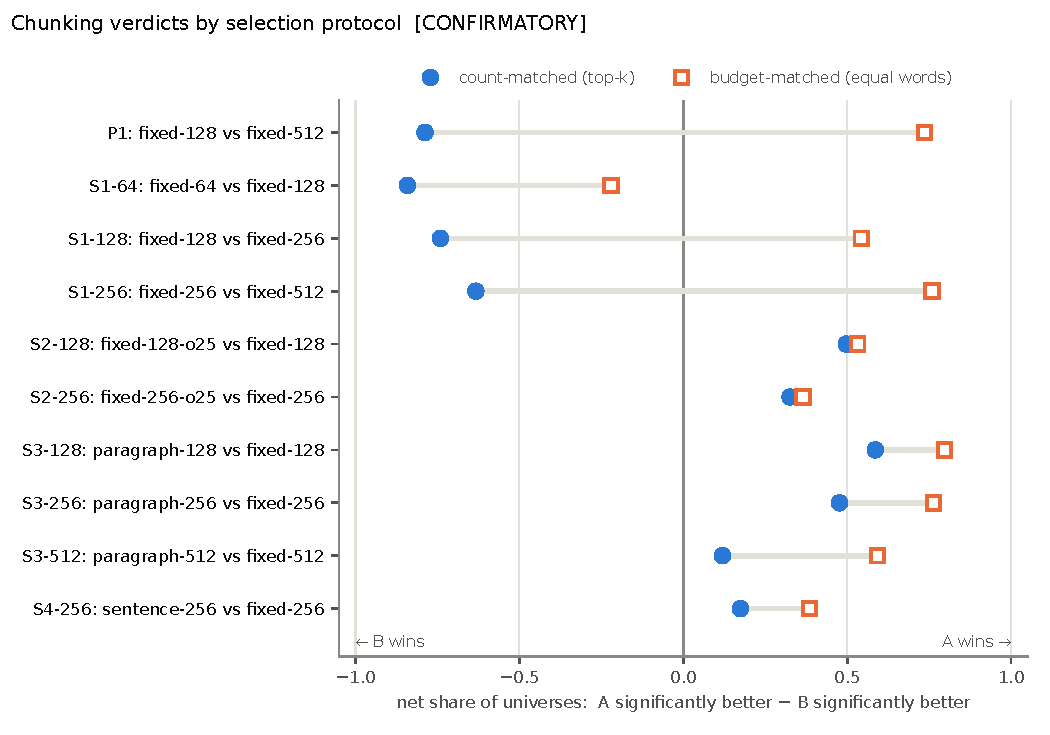
\includegraphics[width=0.92\linewidth]{figures/verdict_dumbbell.pdf}
\caption{Study 1 net support shares, $s_P(A)-s_P(B)$, for selected contrasts on the held-out split. Filled circles show
count matching; open squares show word-budget matching. A move to the right is a relative shift toward A, not
necessarily a reversal of the favoured arm.}
\label{fig:study1}
\end{figure}

% Generated by manuscript/make_tables.py from logged results. Do not edit by hand.
\begin{table*}[t]\centering\footnotesize
\caption{Study~1: share of universes (\%) whose 95\% paired-bootstrap CI supports arm A or arm B, per claim and selection protocol (confirmatory split); the remainder is inconclusive. Budget-matched universes use the admissible budgets $B \ge$ the larger chunk size. $n$ = number of universes.}\label{tab:e1claims}
\begin{tabular}{@{}lllrrrrrr@{}}\toprule
Claim & Role & A vs B & A (count) & B (count) & $n$ & A (budget) & B (budget) & $n$\\\midrule
P1 & primary & \texttt{fixed-128} vs \texttt{fixed-512} & 0.0 & 78.8 & 768 & 81.2 & 7.6 & 576\\
\midrule
S1-64 & secondary & \texttt{fixed-64} vs \texttt{fixed-128} & 0.0 & 84.1 & 768 & 20.0 & 42.1 & 960\\
S1-128 & secondary & \texttt{fixed-128} vs \texttt{fixed-256} & 0.0 & 74.1 & 768 & 60.5 & 6.2 & 768\\
S1-256 & secondary & \texttt{fixed-256} vs \texttt{fixed-512} & 0.0 & 63.3 & 768 & 78.0 & 2.1 & 576\\
\midrule
S2-64 & secondary & \texttt{fixed-64-o25} vs \texttt{fixed-64} & 52.5 & 1.7 & 768 & 54.8 & 1.8 & 960\\
S2-128 & secondary & \texttt{fixed-128-o25} vs \texttt{fixed-128} & 51.6 & 1.8 & 768 & 55.1 & 1.9 & 960\\
S2-256 & secondary & \texttt{fixed-256-o25} vs \texttt{fixed-256} & 36.1 & 3.5 & 768 & 39.8 & 3.3 & 768\\
S2-512 & secondary & \texttt{fixed-512-o25} vs \texttt{fixed-512} & 9.5 & 9.0 & 768 & 11.8 & 6.8 & 576\\
\midrule
S3-64 & secondary & \texttt{paragraph-64} vs \texttt{fixed-64} & 62.2 & 5.7 & 768 & 75.5 & 0.0 & 960\\
S3-128 & secondary & \texttt{paragraph-128} vs \texttt{fixed-128} & 59.8 & 1.2 & 768 & 79.7 & 0.0 & 960\\
S3-256 & secondary & \texttt{paragraph-256} vs \texttt{fixed-256} & 50.1 & 2.5 & 768 & 76.8 & 0.5 & 768\\
S3-512 & secondary & \texttt{paragraph-512} vs \texttt{fixed-512} & 13.7 & 1.7 & 768 & 60.9 & 1.7 & 576\\
\midrule
S4-64 & exploratory & \texttt{sentence-64} vs \texttt{fixed-64} & 58.9 & 6.1 & 768 & 69.5 & 0.4 & 960\\
S4-128 & exploratory & \texttt{sentence-128} vs \texttt{fixed-128} & 50.1 & 0.8 & 768 & 57.6 & 0.0 & 960\\
S4-256 & exploratory & \texttt{sentence-256} vs \texttt{fixed-256} & 19.0 & 1.6 & 768 & 38.5 & 0.0 & 768\\
S4-512 & exploratory & \texttt{sentence-512} vs \texttt{fixed-512} & 6.1 & 0.5 & 768 & 20.8 & 0.3 & 576\\
\bottomrule\end{tabular}
\end{table*}


The decline holds under all five sensitivity analyses (Table~\ref{tab:e1sens}): \SensBHEst\pp{} after multiplicity
adjustment, \SensNoSquadEst\pp{} without SQuAD, \SensDefRetEst\pp{} with the default retriever,
\SensClusterEst\pp{} under the document-cluster bootstrap, and \SensAllBudgetsEst\pp{} with all budgets.

Figure~\ref{fig:p1curve} shows the coverage specification curve. The mean P1 difference changes sign between the
protocols in each collection (Table~\ref{tab:e1bydataset}). The strength of the verdict pattern nevertheless varies:
CUAD has relatively few decisive count-matched settings, while Qasper has a mixture of budget-matched verdicts and a
small positive average difference. The overall shift should not obscure this heterogeneity.

\begin{figure}[tb]
\centering
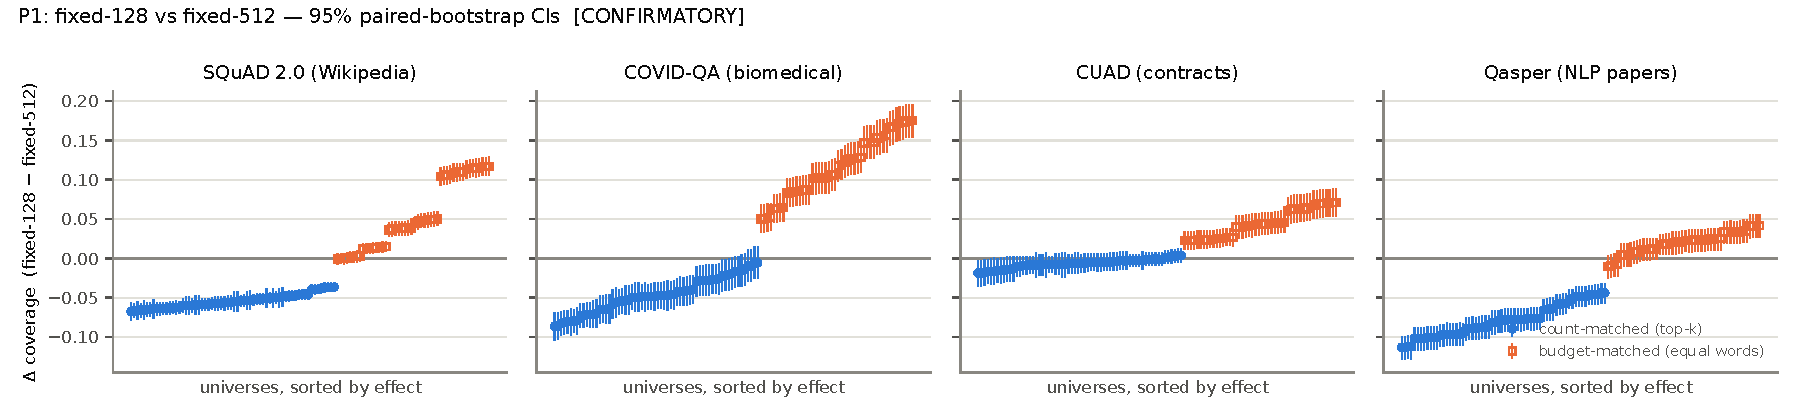
\includegraphics[width=\linewidth]{figures/speccurve_P1_coverage.pdf}
\caption{P1 coverage differences, \chunk{fixed-128} minus \chunk{fixed-512}, with 95\% paired-bootstrap intervals.
Universes are sorted by effect within each dataset.}
\label{fig:p1curve}
\end{figure}

\paragraph{Overlap and structure.}
The S2 overlap contrasts move much less than P1. For S2-128, support for overlap changes from
\StwoOneTwoEightCountA\% to \StwoOneTwoEightBudgetA\%; for S2-256, from \StwoTwoFiveSixCountA\% to
\StwoTwoFiveSixBudgetA\%. These are comparisons at the same cap, but they are not exact equal-length controls: terminal
chunks produce slightly different realised means, and overlap changes how much unique text is covered for a given
charged budget. Their relative stability is consistent with the text-volume explanation without uniquely identifying
it.

For S3-256, paragraph-packing support increases by \HOneBEst\pp{} (95\% CI [\HOneBLo, \HOneBHi]); H1b is
\HOneBVerdict. Paragraph chunks are shorter on average than fixed windows of the same cap (Table~\ref{tab:chunklen}).
Matching the budget removes the unequal allowance in word occurrences, although boundary quality, ranking and
truncation still differ.

Not every contrast reverses. For S1-64, the 128-word arm is supported in \SoneSixFourCountB\% of count-matched and
still \SoneSixFourBudgetB\% of budget-matched universes, against \SoneSixFourBudgetA\% for the 64-word arm. The
defensible generalisation is substantial protocol sensitivity and a movement toward shorter arms, not a universal
advantage for the smallest chunk size.

\paragraph{Dataset dependence and approximate power.}
For S3-256 under budget matching, dataset has $\eta^2=\HTwoDatasetEta$, compared with \HTwoRetrieverEta{} for the
retriever configuration, and is the largest factor in \HTwoFraction\% of bootstrap replicates
(Table~\ref{tab:e1h2}); H2 is \HTwoVerdict. This is a decomposition of mean score differences within the chosen grid,
not a causal explanation of every verdict.

For the S2/S3 budget-matched universes, \HThreeShare\% have an estimated requirement above 500 paired queries, with
median \HThreeMedianN{} (Table~\ref{tab:e1h3}); H3 is \HThreeVerdict. Because multiple queries can share a document,
these quantities should not be read as guaranteed operating characteristics for a new evaluation.
Table~\ref{tab:h} summarises all hypothesis outcomes.

\begin{table}[tb]\centering\small
\caption{Pre-registered hypotheses and outcomes on the held-out split (\EoneNq{} queries). Share changes are
percentage points (pp) of universes, not score improvements; intervals use the joint query bootstrap.}\label{tab:h}
\begin{tabular}{@{}llrlr@{}}\toprule
ID & Statement (short) & Estimate & 95\% CI & Verdict\\\midrule
H1 (primary) & fixed-512 share falls, count $\to$ budget & \HOneEst\pp & [\HOneLo, \HOneHi] & \HOneVerdict\\
H1b & paragraph-256 share rises, count $\to$ budget & \HOneBEst\pp & [\HOneBLo, \HOneBHi] & \HOneBVerdict\\
H2 & dataset explains most variance in $\Delta$ & $\eta^2$ \HTwoDatasetEta & largest in \HTwoFraction\% & \HTwoVerdict\\
H3 & $>$50\% of universes need $n>500$ & \HThreeShare\% & median $n$ \HThreeMedianN & \HThreeVerdict\\\midrule
H4 (primary, 1b) & shorter-arm share rises, semantic-bp & \HFourEst\pp & [\HFourLo, \HFourHi] & \HFourVerdict\\
H4b & same, semantic clustering & \HFourBEst\pp & [\HFourBLo, \HFourBHi] & \HFourBVerdict\\
H5 & dense: fixed-512 share falls & \HFiveEst\pp & [\HFiveLo, \HFiveHi] & \HFiveVerdict\\
H5b$^\dagger$ & dense: fixed-128 share rises & \HFiveBEst\pp & [\HFiveBLo, \HFiveBHi] & \HFiveBVerdict\\\bottomrule
\end{tabular}\\[2pt]
\footnotesize $^\dagger$Added after the exploratory pilot, before the held-out run (disclosed amendment); H5 is the
original test.
\end{table}

\section{Study 1b: semantic chunkers and dense retrieval}\label{sec:study1b}
\subsection{Design and relation to Study 1}
Study 1b reuses the collections, held-out split, metrics and verdict procedure. It extends the evaluated
configurations; it is not an independent replication on new data. Its pre-registration was frozen as version 1.0 at
commit Study 1b freeze record (19 October 2026), after an exploratory pilot on the exploratory split only and before the
held-out run.

\paragraph{Semantic breakpoint chunking.}
The \chunk{semantic-bp} arm embeds sentences individually. A boundary is inserted when the cosine distance between
adjacent sentences exceeds the document's 95th percentile of such distances, using linear interpolation. A
single-sentence document forms one chunk. Sentences longer than 512 words are split first, and groups exceeding 512
words are repacked using the sentence rule. This percentile is a fixed library-default choice, not a value tuned on
the data or taken from Qu et al.'s tested settings~\citeL{qu2025semanticchunking}.

\paragraph{Semantic clustering.}
The \chunk{semantic-cl} arm uses a positional and semantic distance of the form introduced by Qu et
al.~\citeL{qu2025semanticchunking}:
\begin{align}
 d(i,j)&=\lambda d_{\mathrm{pos}}(i,j)+(1-\lambda)d_{\mathrm{cos}}(i,j),\\
 d_{\mathrm{pos}}(i,j)&=|i-j|/n,\qquad
 d_{\mathrm{cos}}(i,j)=1-\max\{\cos(e_i,e_j),0\}.
\end{align}
Here $n$ is the number of sentences and $e_i$ their embeddings. We set $\lambda=0.5$, consider pairs with $d\leq0.5$
in increasing-distance order, break ties by sentence indices, and merge clusters only if their combined length
remains at most 512 words. A chunk can therefore contain non-adjacent text, concatenated in document order. This
capped procedure is an adaptation of the chunker family, not an exact reimplementation.

Both semantic arms use the same encoder as the dense retriever. Each is compared with \chunk{fixed-128},
\chunk{fixed-256} and \chunk{fixed-512}; these contrasts are denoted S5 and S6. Breakpoint means range from \SemBpMin{}
to \SemBpMax{} words across the datasets; clustering means range from \SemClMin{} to \SemClMax, with at least
\SemClNoncontigMin\% of clustering chunks non-contiguous (Table~\ref{tab:chunklen}). The clustering configuration is
therefore close to its cap and should not stand for all semantic-clustering choices.

\paragraph{Retrieval and estimands.}
The extension uses default BM25 and BGE-M3 dense retrieval~\citeL{chen2024bgem3} with normalised embeddings, cosine
ranking, a maximum input length of 8,192 tokens and half precision on one GPU. Chunks are capped at 512 words, far
below that limit; token counts were not logged.

For each dataset and contrast, the shorter arm is the one with the smaller corpus-average chunk length, computed from
chunk statistics before any retrieval metric. The breakpoint arm is longer than the 128- and 256-word fixed arms and
shorter than the 512-word arm. All Study 1b budgets are 512, 1,024 or 2,048 words. Pooling both retrievers gives
\SfiveUniversesCount{} count-matched and \SfiveUniversesBudget{} budget-matched universes per S5/S6 contrast;
dense-only P1 has \PoneDenseUniversesCount{} and \PoneDenseUniversesBudget.

H4 predicts that the shorter arm's support share increases by at least 20 percentage points for breakpoint
comparisons, pooled across fixed sizes and retrievers. H4b sets a 10-point threshold for clustering comparisons. H5
retains Study 1's larger-arm formulation: support for \chunk{fixed-512} should fall by at least 20 points under dense
retrieval. The pilot showed that the larger arm rarely won with dense retrieval even under count matching, which puts
a floor under H5's possible decline; this motivated H5b, a 20-point increase in support for the shorter arm. The
amendment changes the estimand, was made before the held-out run, and is reported separately; H5 remains the
original test.

\subsection{Results}
For breakpoint comparisons, support for the shorter arm rises from \HFourCount\% to \HFourBudget\%, a gain of
\HFourEst\pp{} (95\% CI [\HFourLo, \HFourHi]); H4 is \HFourVerdict. The gain is \HFourBmOnlyEst\pp{} with BM25 and
\HFourDenseOnlyEst\pp{} with dense retrieval; the remaining sensitivity analyses are in Table~\ref{tab:e3sens}.

These pooled shorter-arm shares should not be confused with support for the semantic arm in every contrast. Against
\chunk{fixed-128}, the breakpoint arm is supported in \SfiveOneTwoEightCountSem\% of count-matched settings and
\SfiveOneTwoEightBudgetSem\% of budget-matched settings. Against \chunk{fixed-512}, where breakpoint chunks are
shorter, semantic-arm support instead increases (Table~\ref{tab:e3claims}, Figure~\ref{fig:study1b}). Relative length
and the operating protocol are therefore central to interpreting a semantic-versus-fixed comparison, without
establishing that length alone determines its outcome.

\begin{figure}[tb]
\centering
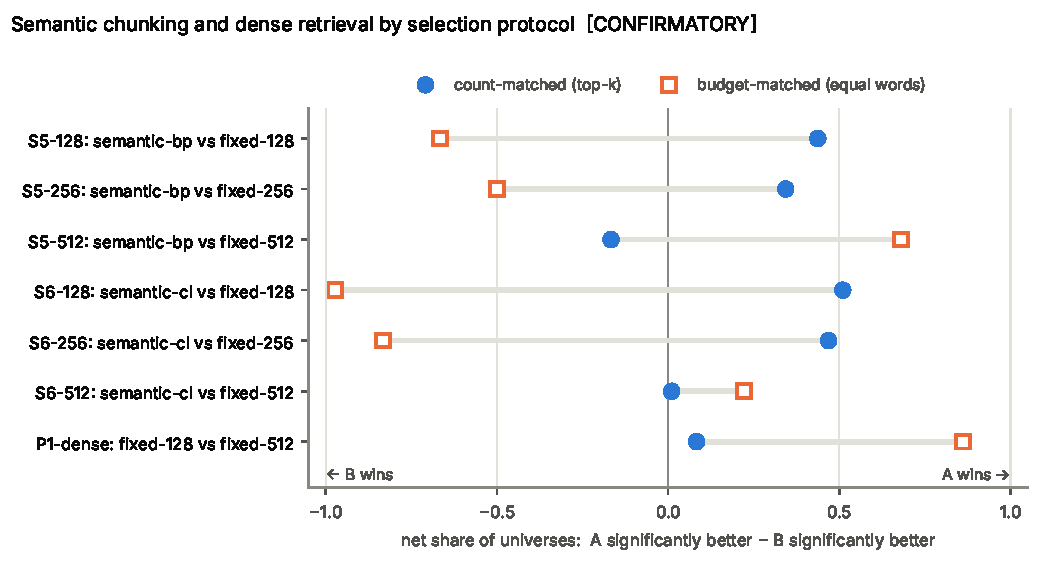
\includegraphics[width=0.94\linewidth]{figures/study1b_dumbbell.pdf}
\caption{Study 1b net support shares. S5 and S6 pool the default BM25 and dense retrievers; P1-dense uses only BGE-M3.
Arm definitions are fixed along each row. Rightward movement is toward A and must be interpreted with the pair's
relative chunk lengths.}
\label{fig:study1b}
\end{figure}

% Generated by manuscript/make_tables.py from logged results. Do not edit by hand.
\begin{table}[t]\centering\footnotesize
\caption{Study~1b: share of universes (\%) supporting arm A or B per claim and protocol (confirmatory). S5/S6 pool BM25 and dense retrieval; P1-dense uses the dense retriever only. Admissible budgets $B \in \{512, 1024, 2048\}$. The S5/S6 rows are the quantity reported by semantic-chunking studies (planned descriptive analysis g).}\label{tab:e3claims}
\begin{tabular}{@{}llrrrrrr@{}}\toprule
Claim & A vs B & A (count) & B (count) & $n$ & A (budget) & B (budget) & $n$\\\midrule
S5-128 & \texttt{semantic-bp} vs \texttt{fixed-128} & 60.4 & 16.7 & 96 & 8.3 & 75.0 & 72\\
S5-256 & \texttt{semantic-bp} vs \texttt{fixed-256} & 38.5 & 4.2 & 96 & 1.4 & 51.4 & 72\\
S5-512 & \texttt{semantic-bp} vs \texttt{fixed-512} & 7.3 & 24.0 & 96 & 68.1 & 0.0 & 72\\
\midrule
S6-128 & \texttt{semantic-cl} vs \texttt{fixed-128} & 53.1 & 2.1 & 96 & 0.0 & 97.2 & 72\\
S6-256 & \texttt{semantic-cl} vs \texttt{fixed-256} & 46.9 & 0.0 & 96 & 0.0 & 83.3 & 72\\
S6-512 & \texttt{semantic-cl} vs \texttt{fixed-512} & 18.8 & 17.7 & 96 & 33.3 & 11.1 & 72\\
\midrule
P1-dense & \texttt{fixed-128} vs \texttt{fixed-512} & 33.3 & 25.0 & 48 & 91.7 & 5.6 & 36\\
\bottomrule\end{tabular}
\end{table}


For clustering, shorter-arm support rises from \HFourBCount\% to \HFourBBudget\%, a gain of \HFourBEst\pp{} (95\% CI
[\HFourBLo, \HFourBHi]); H4b is \HFourBVerdict{} for this configuration. The result does not identify which part of the
clustering procedure, its length distribution or its non-contiguity is responsible.

For dense P1, support for the larger fixed arm falls from \HFiveCountFiveTwelve\% to \HFiveBudgetFiveTwelve\%. The
decline is \HFiveEst\pp{} (95\% CI [\HFiveLo, \HFiveHi]). Its point estimate does not reach 20 points, while the
interval does not place the entire effect below that threshold, so H5 is \HFiveVerdict{} under the stated rule;
excluding zero alone does not make it supported. The amended shorter-arm statistic rises from \HFiveBCount\% to
\HFiveBBudget\%, a gain of \HFiveBEst\pp{} (95\% CI [\HFiveBLo, \HFiveBHi]); H5b is \HFiveBVerdict. Both outcomes are
reported.

\section{Exploratory answer-quality evaluation}\label{sec:tier2}
\subsection{Setup and contrast}
The answer-quality check uses a seeded sample (seed 20261019) of 50 held-out queries per dataset, 200 in total. It
evaluates P1 and S3-256 with the default BM25 retriever, top-5 selection and a 1,024-word budget. Four chunkings and
two operating points give 1,600 generation jobs. The analysis plan was committed before any generation
(\path{experiments/E2_generation/ANALYSIS_PLAN.md}); the check is exploratory and cannot change any hypothesis verdict.

The reader is Qwen3-4B~\citeL{qwen2025qwen3}, a Q4\_K\_M quantised GGUF file run with llama.cpp. Decoding disables
thinking, is greedy and permits at most 256 output tokens. The prompt supplies numbered passages and the question, with
a fixed instruction asking for the shortest supported answer or ``unanswerable'' (Appendix~\ref{app:impl}). Answers
are scored by SQuAD-style token F1 and exact match against the reference answers.

For a query and contrast, let $\Delta_q(o)$ be the difference between arms A and B at operating point $o$. The
difference-in-differences is
\begin{equation}
 \mathrm{DiD}_q=\Delta_q(B=1024)-\Delta_q(k=5).
 \label{eq:did}
\end{equation}
A positive DiD indicates a relative gain for A on changing protocol; it does not establish that A has a higher absolute
score at the budget-matched point. The pooled estimate gives each dataset equal weight, with 2,000 stratified bootstrap
resamples. We report the same contrast for exact match and retrieval coverage on the same queries, and the minimum
detectable effect (MDE).

\subsection{Results and interpretation}
All 1,600 jobs completed. The coverage DiD is \EtwoPoneCov{} (95\% CI [\EtwoPoneCovLo, \EtwoPoneCovHi]) for P1 and
\EtwoSthreeCov{} ([\EtwoSthreeCovLo, \EtwoSthreeCovHi]) for S3-256. These are positive protocol interactions for
retrieval coverage, consistent with Study 1, though not by themselves proof that the within-protocol ordering reverses
in this smaller sample.

The answer-F1 DiDs are \EtwoPoneFone{} ([\EtwoPoneFoneLo, \EtwoPoneFoneHi]) and \EtwoSthreeFone{}
([\EtwoSthreeFoneLo, \EtwoSthreeFoneHi]), respectively. Both intervals include zero. The check therefore fails to
establish the predicted positive answer-F1 interaction; it does not establish the absence of an effect or equivalence
between protocols.

For P1, exact match has a negative DiD of \EtwoPoneEm{} ([\EtwoPoneEmLo, \EtwoPoneEmHi]). The arm-level means show
what this interaction consists of: averaged over datasets, the 128-word arm has the higher exact match at top-5
(\EtwoEmOneTwoEightCount{} vs \EtwoEmFiveTwelveCount) and the 512-word arm at the 1,024-word budget
(\EtwoEmFiveTwelveBudget{} vs \EtwoEmOneTwoEightBudget). These cell means are descriptive and carry no separate
interval. Table~\ref{tab:e2did} reports the per-dataset and pooled results, including this directionally contrary
finding.

% Generated by manuscript/make_tables.py from logged results. Do not edit by hand.
\begin{table*}[t]\centering\footnotesize
\caption{Answer-quality check (exploratory; written analysis plan\artifactref{experiments/E2_generation/ANALYSIS_PLAN.md}): difference-in-differences DiD $= \Delta(B{=}1{,}024) - \Delta(k{=}5)$, $\Delta$ = metric(A) $-$ metric(B), with 95\% bootstrap CIs (2{,}000 resamples; pooled: stratified by dataset). The retrieval mechanism predicts DiD $> 0$; an interval that includes 0 does not establish the absence of an effect. 50 queries per dataset; reader Qwen3-4B (Q4\_K\_M, greedy).}\label{tab:e2did}
\begin{tabular}{@{}llrrr@{}}\toprule
Claim & Dataset & Answer F1 & Exact match & Coverage\\\midrule
P1 & SQuAD 2.0 & $-$0.122 [$-$0.245, +0.009] & $-$0.160 [$-$0.300, 0.000] & +0.120 [+0.040, +0.220]\\
 & COVID-QA & $-$0.006 [$-$0.101, +0.090] & $-$0.060 [$-$0.160, +0.020] & +0.110 [+0.040, +0.200]\\
 & CUAD & $-$0.001 [$-$0.031, +0.033] & 0.000 [0.000, 0.000] & +0.020 [0.000, +0.060]\\
 & Qasper & +0.060 [$-$0.015, +0.158] & 0.000 [$-$0.060, +0.060] & +0.106 [+0.020, +0.214]\\
 & Pooled (stratified) & $-$0.017 [$-$0.065, +0.033] & $-$0.055 [$-$0.100, $-$0.010] & +0.089 [+0.050, +0.132]\\
 & Minimum detectable effect & 0.068 & 0.066 & 0.059\\
\midrule
S3-256 & SQuAD 2.0 & $-$0.027 [$-$0.104, +0.049] & $-$0.060 [$-$0.160, +0.060] & +0.060 [0.000, +0.140]\\
 & COVID-QA & +0.005 [$-$0.050, +0.066] & $-$0.020 [$-$0.100, +0.040] & +0.060 [0.000, +0.140]\\
 & CUAD & $-$0.008 [$-$0.027, +0.012] & 0.000 [0.000, 0.000] & 0.000 [0.000, 0.000]\\
 & Qasper & +0.045 [$-$0.017, +0.117] & +0.020 [0.000, +0.060] & +0.020 [0.000, +0.060]\\
 & Pooled (stratified) & +0.004 [$-$0.024, +0.036] & $-$0.015 [$-$0.050, +0.020] & +0.035 [+0.015, +0.060]\\
 & Minimum detectable effect & 0.044 & 0.051 & 0.036\\
\bottomrule\end{tabular}
\end{table*}


The P1 answer-F1 MDE is \EtwoPoneFoneMde. An MDE describes sensitivity under a power calculation; it is not an observed
exclusion bound, so we do not claim that the experiment rules out all effects above that value. The confidence
intervals, limited sample and single-reader setting define the evidential scope.

Completion does not imply that every response was unrestricted by the output cap: \EtwoTruncCuad{} of
\EtwoJobsCuad{} CUAD outputs and \EtwoTruncQasper{} of \EtwoJobsQasper{} Qasper outputs reached the 256-token cap
(Table~\ref{tab:e2diag}). The cap plausibly affects answer metrics for long reference answers, but its contribution has
not been isolated. One exploratory, not pre-specified observation: in SQuAD at the 1,024-word budget, answer F1 is
\EtwoSquadFiveTwelveBudgetFone{} with two 512-word passages and \EtwoSquadOneTwoEightBudgetFone{} with eight 128-word
passages, at similar retrieval coverage (\EtwoSquadFiveTwelveBudgetCov{} vs \EtwoSquadOneTwoEightBudgetCov). Passage
continuity is one possible explanation, to be tested rather than assumed.

\section{A provisional audit of chunking evaluations}\label{sec:audit}
We coded \AuditN{} empirical chunking studies published or posted in 2024--2026. Candidates were identified by logged
web searches before any full text was read (\path{literature/protocol_audit/candidates.csv}), and the inclusion rule
and coding scheme were fixed in advance (\path{literature/protocol_audit/PROTOCOL.md}). A study is included if it
empirically compares at least two chunkings on a retrieval or answer metric and states a conclusion about that
comparison. \todo{state the search sources, queries and dates, and the number of hits screened, from the search log.}

Each study is coded for the protocol of its headline comparison (fixed count, matched budget, other, unclear), whether
its arms differ in chunk length, whether the retrieved text volume is reported, whether uncertainty is reported for a
chunking contrast, and the metric type. A fixed rule (\path{analyze_audit.py}) derives an exposure label: a study is
\emph{exposed} if its headline comparison is count-based and its arms differ in chunk length. One study coded
protocol ``other'' is treated as count-based because it scores reciprocal rank over chunks of different granularity
(Garrido-Lestache Belinchon and Garrido-Lestache Belinchon~\citeL{garrido2026chunksize}).

The table contains \AuditFixedK{} fixed-count studies, \AuditBudget{} matched-budget study and \AuditUncertainty{}
studies reporting a confidence interval or significance test for a chunking contrast; \AuditExposed{} are labelled
exposed, one of which reports its retrieved text volume (Table~\ref{tab:audit}, Appendix~\ref{app:audit}). These are
counts from a single coder whose work was AI-assisted; independent double-coding of a random 30\% subsample is
pending, so no reliability coefficient is available yet. \todo{report Cohen's $\kappa$ after the blind double-coding.}

For completeness, \AuditExposed/\AuditN{} is \AuditExposedPct\%, with Wilson interval [\AuditExposedLo,
\AuditExposedHi]\%. That interval cannot account for coding errors, incomplete screening or a non-probability sample
of papers, and we do not use it as a headline estimate of the literature. Exposure to an uncontrolled quantity does not
show that an audited study's substantive conclusion is wrong: its metric and practical comparison objective also
matter.

\section{Discussion}\label{sec:discussion}
\subsection{What the protocol sensitivity establishes}
The primary result shows that an apparent preference for larger chunks can change substantially when the comparison
fixes word occurrences rather than chunk count. The smaller shifts in same-cap overlap contrasts and the direction of
the semantic comparisons are consistent with retrieved-text allowance being an important component of this
sensitivity. They do not isolate text volume as the sole causal mechanism: segmentation changes ranking, boundary
placement, redundancy and passage continuity at the same time.

Budget matching removes one difference between systems: the allowance in counted words. It does not equalise unique
evidence, model-token usage, indexing cost, latency or the reader's ability to use the selected context. Truncating a
ranked chunk can also change its semantic completeness. These choices define the question the protocol answers.

A fixed-$k$ comparison remains appropriate when deployment genuinely fixes the number of passages; a fixed-budget
comparison is appropriate when the amount of retrieved text is the relevant constraint. Disagreement between their
verdicts is not a contradiction. It means that the practical preference is conditional on an operating constraint,
rather than an intrinsic property of the chunker.

\subsection{Retriever and reader dependence}
With BGE-M3, the larger fixed arm is already less dominant under count matching than in the lexical grid. It is
plausible that combining more topics in one embedding affects ranking, but the experiments do not test that mechanism
directly, so we report it as observed configuration dependence.

The answer check provides a second boundary. More recovered gold text and better generated answers are not
interchangeable outcomes. Positive coverage interactions coexist with uncertain answer-F1 interactions and a negative
exact-match interaction for P1. Passage continuity, irrelevant context, answer normalisation and output truncation are
possible explanations, not demonstrated mediators; resolving them requires controlled comparisons.

\subsection{Reporting implications}
A useful chunking report identifies the chunker, nominal cap, realised length distribution, overlap policy, retriever
and metric. It states the number of selected passages and the retrieved word or token budget, including how duplicates
and the last chunk are handled. Reporting both count-matched and budget-matched results makes the operating constraint
explicit rather than hiding it in a retrieval parameter.

Statistical summaries need clear denominators and estimands. Support shares should be accompanied by their universe
counts, uncertainty procedure and the grid to which they refer. A difference in support shares should not be called a
flip rate unless universes are paired and a transition statistic is computed. Query-level and document-level
uncertainty answer different sampling questions and should be identified accordingly.

Finally, retrieval and answer evaluations should be reported separately. A coverage gain can motivate an answer-level
experiment, but it cannot replace one; an answer-level difference should include enough information about text volume
and passage count to explain the operating condition under which it occurs.

\section{Limitations and threats to validity}\label{sec:limitations}
\paragraph{Construct validity.}
The three span metrics are coverage-oriented, reward any or the best-covered evidence span, and do not penalise
irrelevant retrieved text. Results need not transfer to retrieval precision, evidence F1, factuality or complete
multi-hop evidence acquisition. Budgets use words rather than model tokens, while evidence overlap uses characters.
Charging repeated words does not equalise unique context.

\paragraph{Internal validity.}
Sentence boundaries are rule-based, paragraph boundaries use blank lines, and the final selected chunk may be
truncated. The semantic arms use one setting each, fixed in advance; clustering yields mostly non-contiguous chunks
near the cap, which limits its interpretation as a general test of semantic clustering. Same-cap overlap comparisons
have slightly different realised lengths and redundancy, so they are not exact mechanistic controls.

\paragraph{Statistical validity.}
Universes reuse queries and are not independent replications. Joint query resampling addresses shared-query
dependence but does not sample new datasets; query nesting in documents is addressed by a designated sensitivity
analysis. The joint procedure approximates inner confidence intervals, and the significance threshold helps
determine the support shares. The grids contain different numbers of operating points across protocols and contrasts;
their weights are design choices. The H3 estimates are approximate power calculations, and the exploratory answer
results are not a multiplicity-controlled family of confirmatory tests.

\paragraph{External validity.}
The study covers four English extractive or evidence-annotated question-answering collections, one lexical family and
one dense encoder. Study 1b reuses the same held-out queries. The generation check has one quantised 4B reader and 200
sampled queries, with an output cap that truncated some answers. Other languages, long-form tasks, rerankers,
readers, encoders and cost constraints remain outside the demonstrated scope.

\paragraph{Pre-registration and audit.}
H5b is a disclosed post-pilot amendment, and one sensitivity interval was corrected after the held-out run
(Appendix~\ref{app:deviations}); neither changes a confirmatory estimate or verdict. The audit is provisional and is
unsuitable for a definitive claim about the prevalence of the problem.

\section{Conclusion}
Chunking evaluation is highly sensitive to the retrieval-selection protocol. In the primary lexical comparison,
support for 512-word chunks declines by \HOneEst\pp{} when moving from count matching to admissible word-budget
matching; in the semantic-breakpoint comparisons, the shorter arm gains \HFourEst\pp{} of support. These are different
estimands, both conditional on the evaluated grid. The original dense-retrieval hypothesis is inconclusive, while its
disclosed shorter-arm amendment is supported. The exploratory answer evaluation does not establish a corresponding
answer-F1 effect and shows a contrary exact-match interaction for the primary contrast. The practical conclusion is
therefore narrower than a recommendation for one chunk size or chunker: comparisons should disclose both retrieval
depth and text budget, and retrieval-level evidence should not be presented as an answer-quality result.

\section{Reproducibility}\label{sec:reproducibility}
Code, data manifests with SHA-256 hashes, both pre-registrations with their freeze commits (Study 1 freeze record,
Study 1b freeze record) and deviation logs, run manifests (commit, package versions, hardware) and all per-query results and
generations are available at \url{https://github.com/swaroopchandrashekar13/rag-research}. Every number in this paper is generated from the
logged results by \path{manuscript/make_numbers.py} and every results table by \path{manuscript/make_tables.py}.


\bibliographystyle{plainnat}
\bibliography{refs}

\clearpage
\appendix
\section{Deviations from the pre-registrations}\label{app:deviations}
Table~\ref{tab:deviations} summarises the logged deviations (\path{research/preregistration.md}, Section 9;
\path{research/preregistration_study1b.md}, Section 8). The post-run interval correction and the post-pilot H5b
amendment are listed rather than removed.

\begin{table}[htbp]\centering\footnotesize
\caption{Deviations from the pre-registrations (summary of the logged tables).}\label{tab:deviations}
\begin{tabular}{@{}p{1.6cm}p{6.4cm}p{6.4cm}@{}}\toprule
Study & Deviation & Timing and effect\\\midrule
Study 1 & Budget-matched universes restricted to $B \ge \max(W_A, W_B)$; all budgets moved to a sensitivity analysis &
Before any pilot or held-out run; a smoke test showed that smaller budgets force truncation of the top chunk\\
Study 1 & Document-cluster bootstrap sensitivity analysis added & Before any run; queries are nested in few SQuAD
articles\\
Study 1 & Wording of the $\eta^2$ method aligned with the analytic implementation (identical for the balanced design)
& After the pilot, before freezing; same estimands and thresholds\\
Study 1 & Bug fix: the document-cluster sensitivity analysis used query-level resampling for its interval & After the
held-out run; only that sensitivity interval changed (by about one point); no estimate or verdict changed\\
Answer check & Reader changed from a hosted API model to a local open model (Qwen3-4B); scope fixed to 50 queries per
dataset, $k=5$ and $B=1{,}024$ & Before any analysed generation; API quota. The check is exploratory\\
Study 1b & Implementation details written down & During implementation, before any pilot output\\
Study 1b & H5b added; H5 kept unchanged & After the exploratory pilot, before the held-out run\\
Study 1b & Clustering defaults kept although clusters fill the 512-word cap & After the pilot; changing them would have
been tuning on outcomes; reported as a limitation\\\bottomrule
\end{tabular}
\end{table}

\section{Implementation record}\label{app:impl}
\paragraph{Dense retrieval.} BGE-M3 at Hugging Face revision \texttt{5617a9f61b02}, \texttt{sentence-transformers}
6.1.0, \texttt{transformers} 5.20.1 and \texttt{torch} 2.14.1; normalised embeddings cached in half precision; ties in
cosine score resolved by the lower chunk index. Half-precision GPU embeddings are not bit-identical to CPU ones; all
Study 1b universes come from one run.

\paragraph{Reader.} Qwen3-4B GGUF (Q4\_K\_M) at Hugging Face commit \texttt{bc640142}, file SHA-256
\texttt{7485fe6f\allowbreak 11af2943\allowbreak 3bc51cab\allowbreak 58009521\allowbreak f205840f\allowbreak
5b4ae3a3\allowbreak 2fa7f92e\allowbreak 8534fdf5}, with \texttt{llama-cpp-python} 0.3.36 on one NVIDIA Tesla T4 GPU;
ChatML prompt with an empty thinking block; temperature 0, top-$k$ 1, seed 7, at most 256 output tokens. The system
instruction is: \emph{``Answer the question using only the numbered passages. Reply with the shortest answer that is
fully supported by the passages, copying the wording from them where possible. If the passages do not contain the
answer, reply exactly: unanswerable''}; the user message lists the passages as ``[1] \dots'' followed by
``Question: \dots\ Answer:''. Before analysis, every stored prompt's SHA-256 was checked against a prompt rebuilt from
the sampled queries, and every row's retrieval metrics against Study 1's measurements for that query (no mismatches).

\FloatBarrier
\section{Additional retrieval results}\label{app:retrieval}
Table~\ref{tab:chunklen} contains corpus-level mean chunk lengths, not per-query retrieved-text measurements.

% Generated by manuscript/make_tables.py from logged results. Do not edit by hand.
\begin{table}[t]\centering\small
\caption{Mean chunk length in words per chunking and dataset (full retrieval corpus), from the run manifests; they depend only on the chunking, not on any retrieval metric. These lengths define the ``shorter arm'' of every Study~1b claim. The fixed chunkings of Study~1b are the same chunks as in Study~1.}\label{tab:chunklen}
\begin{tabular}{@{}lrrrr@{}}\toprule
Chunking & SQuAD 2.0 & COVID-QA & CUAD & Qasper\\\midrule
\texttt{fixed-64} & 64 & 64 & 64 & 63\\
\texttt{fixed-128} & 126 & 126 & 127 & 126\\
\texttt{fixed-256} & 249 & 247 & 252 & 247\\
\texttt{fixed-512} & 485 & 483 & 495 & 477\\
\texttt{fixed-64-o25} & 64 & 64 & 64 & 64\\
\texttt{fixed-128-o25} & 127 & 127 & 127 & 127\\
\texttt{fixed-256-o25} & 252 & 252 & 253 & 251\\
\texttt{fixed-512-o25} & 497 & 494 & 502 & 491\\
\texttt{sentence-64} & 49 & 49 & 46 & 50\\
\texttt{sentence-128} & 111 & 111 & 98 & 113\\
\texttt{sentence-256} & 235 & 234 & 213 & 235\\
\texttt{sentence-512} & 476 & 470 & 453 & 466\\
\texttt{paragraph-64} & 46 & 45 & 41 & 42\\
\texttt{paragraph-128} & 90 & 90 & 85 & 88\\
\texttt{paragraph-256} & 187 & 179 & 174 & 199\\
\texttt{paragraph-512} & 420 & 392 & 379 & 435\\
\midrule
\texttt{semantic-bp} & 293 & 287 & 320 & 278\\
\texttt{semantic-cl} & 456 & 455 & 458 & 452\\
\quad non-contiguous chunks (\%) & 92.5 & 94.1 & 92.0 & 94.7\\
\bottomrule\end{tabular}
\end{table}

% Generated by manuscript/make_tables.py from logged results. Do not edit by hand.
\begin{table}[t]\centering\footnotesize
\caption{Study~1 per dataset: share of universes (\%) supporting arm A or B, and the mean difference $\bar\Delta = $ metric(A) $-$ metric(B) over universes. P1: A = fixed-128, B = fixed-512. S3-256: A = paragraph-256, B = fixed-256.}\label{tab:e1bydataset}
\begin{tabular}{@{}llrrrrrr@{}}\toprule
Claim & Dataset & A (count) & B (count) & $\bar\Delta$ (count) & A (budget) & B (budget) & $\bar\Delta$ (budget)\\\midrule
P1 & SQuAD 2.0 & 0.0 & 100.0 & $-$0.055 & 83.3 & 0.0 & +0.053\\
 & COVID-QA & 0.0 & 89.1 & $-$0.054 & 100.0 & 0.0 & +0.109\\
 & CUAD & 0.0 & 26.0 & $-$0.009 & 97.2 & 0.0 & +0.040\\
 & Qasper & 0.0 & 100.0 & $-$0.093 & 44.4 & 30.6 & +0.002\\
\midrule
S3-256 & SQuAD 2.0 & 69.3 & 0.0 & +0.014 & 100.0 & 0.0 & +0.034\\
 & COVID-QA & 77.1 & 0.0 & +0.028 & 100.0 & 0.0 & +0.058\\
 & CUAD & 1.0 & 9.9 & $-$0.003 & 8.3 & 2.1 & +0.002\\
 & Qasper & 53.1 & 0.0 & +0.019 & 99.0 & 0.0 & +0.030\\
\bottomrule\end{tabular}
\end{table}

% Generated by manuscript/make_tables.py from logged results. Do not edit by hand.
\begin{table}[t]\centering\small
\caption{Study~1, H1 under the planned sensitivity analyses: drop in the share of universes supporting fixed-512 from count- to budget-matched selection, in percentage points (threshold 20). (a) changes the verdict rule and has no joint-bootstrap CI.}\label{tab:e1sens}
\begin{tabular}{@{}lrl@{}}\toprule
Analysis & Estimate (pp) & 95\% CI\\\midrule
Main analysis (as planned) & 71.1 & [64.8, 81.9]\\
\midrule
(a) Benjamini--Hochberg FDR 5\% within claim, protocol and dataset & 68.0 & ---\\
(b) without SQuAD 2.0 & 61.5 & [53.2, 74.8]\\
(c) default retriever only (Lucene, $k_1$=1.5, $b$=0.75, stemmed) & 70.8 & [64.6, 85.4]\\
(d) document-cluster bootstrap & 69.7 & [63.8, 82.0]\\
(e) all budgets, including $B <$ chunk size & 74.2 & [68.3, 84.8]\\
\bottomrule\end{tabular}
\end{table}

% Generated by manuscript/make_tables.py from logged results. Do not edit by hand.
\begin{table}[t]\centering\small
\caption{Study~1, H2: main-effects decomposition of $\Delta_u$ for S3-256 under budget-matched selection.}\label{tab:e1h2}
\begin{tabular}{@{}lr@{}}\toprule
Quantity & Value\\\midrule
$\eta^2$ of dataset & 0.614\\
$\eta^2$ of budget & 0.096\\
$\eta^2$ of retriever & 0.044\\
$\eta^2$ of metric & 0.032\\
dataset largest (share of bootstrap replicates) & 100.0\%\\
\bottomrule\end{tabular}
\end{table}

% Generated by manuscript/make_tables.py from logged results. Do not edit by hand.
\begin{table}[t]\centering\small
\caption{Study~1, H3: paired queries needed to detect $|\delta| = 0.02$ ($\alpha=0.05$ two-sided, power 0.8), $n = ((1.96 + 0.8416)\,\sigma_d / 0.02)^2$, per budget-matched universe.}\label{tab:e1h3}
\begin{tabular}{@{}lrr@{}}\toprule
Claim & Median $n$ & Universes with $n > 500$ (\%)\\\midrule
S2-64 & 1,175 & 82.5\\
S2-128 & 1,162 & 84.8\\
S2-256 & 1,149 & 79.7\\
S2-512 & 1,161 & 78.0\\
S3-64 & 1,498 & 92.5\\
S3-128 & 1,412 & 90.6\\
S3-256 & 1,399 & 86.2\\
S3-512 & 1,248 & 84.7\\
\midrule
All S2 and S3 universes & 1,256 & 85.4\\
\bottomrule\end{tabular}
\end{table}

% Generated by manuscript/make_tables.py from logged results. Do not edit by hand.
\begin{table}[t]\centering\small
\caption{Study~1b, H4 under the planned sensitivity analyses: share of S5 universes (\%) supporting the shorter arm under count- and budget-matched selection, and the difference (pp; threshold 20). Study~1b uses only the default BM25 configuration, so sensitivity (c), the default-retriever restriction, does not apply.}\label{tab:e3sens}
\begin{tabular}{@{}lrrrl@{}}\toprule
Analysis & Count & Budget & Difference & 95\% CI\\\midrule
Main analysis (H4 as planned) & 9.4 & 64.8 & 55.4 & [50.8, 63.1]\\
\midrule
(a) Benjamini--Hochberg FDR 5\% within claim, protocol and dataset & --- & --- & 54.3 & ---\\
(b) without SQuAD 2.0 & 6.9 & 54.9 & 48.0 & [42.7, 58.3]\\
(d) document-cluster bootstrap & 8.0 & 66.7 & 58.7 & [50.0, 63.3]\\
(e) all budgets & 9.4 & 63.1 & 53.7 & [49.7, 60.9]\\
(f) BM25 only & 0.0 & 61.1 & 61.1 & [57.2, 72.5]\\
(f) dense only & 18.8 & 68.5 & 49.8 & [39.1, 58.1]\\
\bottomrule\end{tabular}
\end{table}


\begin{figure}[tb]
\centering
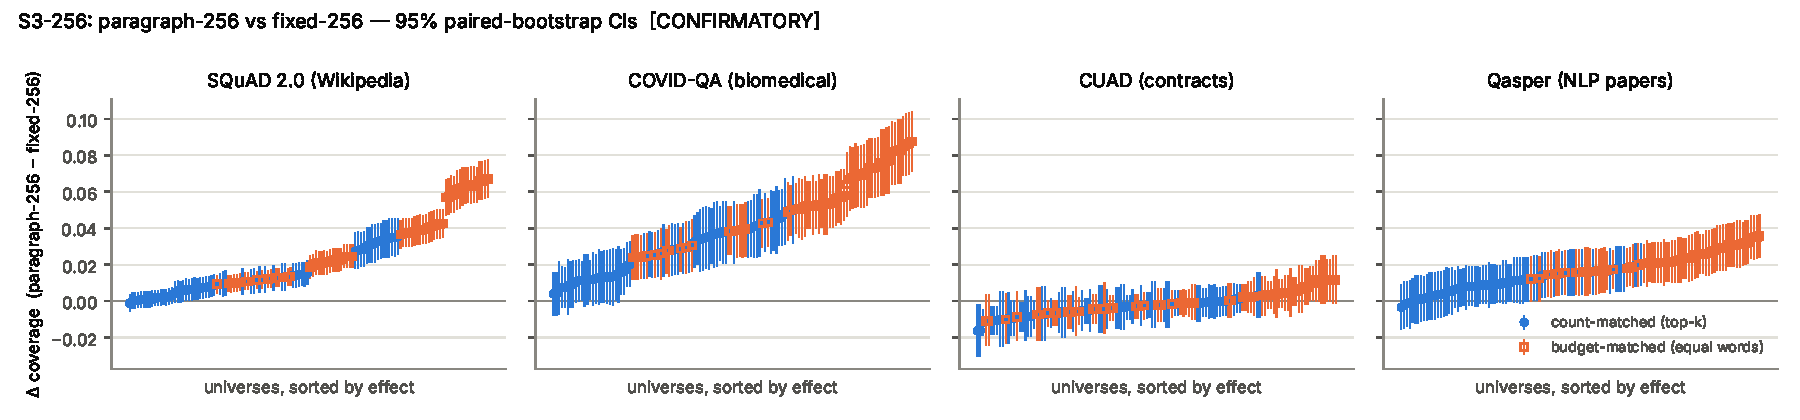
\includegraphics[width=\linewidth]{figures/speccurve_S3-256_coverage.pdf}
\caption{S3-256 coverage specification curve: paragraph packing minus fixed windows, both with a 256-word cap.}
\label{fig:s3curve}
\end{figure}
The S3-256 curves in Figure~\ref{fig:s3curve} accompany the per-dataset results. Near-zero CUAD differences caution
against treating the pooled structure-aware result as uniform across domains.

\FloatBarrier
\section{Generation diagnostics}\label{app:diagnostics}
Table~\ref{tab:e2diag} summarises the generations per dataset. The correlation does not establish a causal relation
between retrieved coverage and answer quality. ``Hit'' denotes at least half of a gold span retrieved, not retrieval of
all evidence needed for an answer.

% Generated by manuscript/make_tables.py from logged results. Do not edit by hand.
\begin{table}[t]\centering\footnotesize
\caption{Answer-quality check, planned diagnostics per dataset (400 generations each): completed jobs, answers truncated at the 256-token cap, share of ``unanswerable'' replies, and the link between retrieval and answers (Pearson correlation of coverage and F1; mean F1 when the gold evidence was / was not at least half retrieved).}\label{tab:e2diag}
\begin{tabular}{@{}lrrrrrr@{}}\toprule
Dataset & Jobs ok & Truncated & Unanswerable (\%) & $r$(coverage, F1) & F1 | hit & F1 | miss\\\midrule
SQuAD 2.0 & 400/400 & 0 & 4.2 & 0.36 & 0.56 & 0.06\\
COVID-QA & 400/400 & 0 & 5.8 & 0.33 & 0.40 & 0.15\\
CUAD & 400/400 & 65 & 15.0 & 0.66 & 0.70 & 0.14\\
Qasper & 400/400 & 2 & 15.8 & 0.53 & 0.37 & 0.08\\
\bottomrule\end{tabular}
\end{table}


\FloatBarrier
\section{Audit records}\label{app:audit}
Table~\ref{tab:audit} reproduces the audit coding, including ``other'', ``unclear'' and ``possibly exposed'' cases,
without recoding. It is not a completed systematic-review result. Beyond the studies discussed in the main text, the
audit covers work on Arabic RAG, cross-granularity chunking, context reconstruction, chunking taxonomies, embedding
sensitivity, academic texts, computational cost, PDF parsing, query-adaptive chunking, chunk size and
logic-aware segmentation~\citeL{arabicrag2025,freechunker2025,reconstructingcontext2025,beyondchunkthenembed2026,chunkembedsensitivity2026,chunkingacademic2026,chunkingcost2026,pdfparsingfin2026,queryadaptivechunking2026,garrido2026chunksize,metachunking2024}.

% Generated by manuscript/make_tables.py from logged results. Do not edit by hand.
\begin{table*}[t]\centering\footnotesize
\caption{Protocol audit: coding of each included study (provisional; see Section~\ref{sec:audit}). Protocol: how arms are compared; Length differs: whether the compared arms produce chunks of different length; Text reported: whether the amount of retrieved text is reported; Uncertainty: for chunking contrasts; Exposure: derived by the audit's coding rules\artifactref{literature/protocol_audit/analyze_audit.py}.}\label{tab:audit}
\begin{tabular}{@{}lllllll@{}}\toprule
Study & Protocol & Length differs & Text reported & Uncertainty & Metric & Exposure\\\midrule
\citeL{qu2025semanticchunking} & fixed $k$ & unclear & no & none & both & possibly exposed\\
\citeL{bhat2025chunksize} & fixed $k$ & yes & no & none & retrieval & exposed\\
\citeL{muthyam2026ragstability} & fixed $k$ & yes & yes & seeds & both & exposed, text reported\\
\citeL{beyondchunkthenembed2026} & fixed $k$ & yes & no & test & retrieval & exposed\\
\citeL{chunkembedsensitivity2026} & fixed $k$ & yes & no & CI & retrieval & exposed\\
\citeL{garrido2026chunksize} & other & yes & no & none & retrieval & exposed\\
\citeL{chunkingcost2026} & fixed $k$ & yes & no & none & both & exposed\\
\citeL{pdfparsingfin2026} & other & unclear & no & none & both & not exposed\\
\citeL{chunkingacademic2026} & unclear & unclear & no & none & both & undeterminable\\
\citeL{reconstructingcontext2025} & other & unclear & no & none & both & not exposed\\
\citeL{hichunk2025} & budget & yes & yes & none & both & not exposed\\
\citeL{metachunking2024} & fixed $k$ & no & no & none & answer & not exposed\\
\citeL{freechunker2025} & fixed $k$ & unclear & no & seeds & answer & possibly exposed\\
\citeL{moc2025} & fixed $k$ & no & no & CI & answer & not exposed\\
\citeL{queryadaptivechunking2026} & fixed $k$ & yes & no & seeds & both & exposed\\
\citeL{arabicrag2025} & unclear & unclear & no & none & both & undeterminable\\
\citeL{jimenoyepes2024financial} & fixed $k$ & yes & no & none & both & exposed\\
\citeL{duarte2024lumberchunker} & fixed $k$ & yes & no & none & both & exposed\\
\citeL{gunther2024latechunking} & other & no & no & none & retrieval & not exposed\\
\bottomrule\end{tabular}
\end{table*}


\end{document}
